\section{IoHT-Framework}\label{sec:three}
\subsection{Layered Architecture}
IoT implementation on large scale leads to challenges such as large number of connected devices and voluminous data having limited processing power and resources.Centralized cloud based IoT is a key that can handle huge data generated by heterogenous devices in an IoT Framework.\\
Although cloud is efficient enough on a large scale,it can cause some latency issues and consume more power which can make a solo cloud more critical at times.To handle the load on cloud,an introduction of Fog is an approach that ensures reliability,energy-efficiency and performance in IoT frameworks\cite{rahmani2018exploiting}\cite{3}.\\

However there still exists QoS issues in order to deal with different kinds of data processing at each layers.The solution to this problem is the five layered fog-based architecture that is capable of handling different kinds of data processing based on the demands in different layers.The introduction of additional layer called "Mist Layer" to the Fog architecture reduces volume of the data that has to be transmitted to IoT devices using rule-based prepocessing which in turn reduces the power consumption,latency and computational complexity of the framework\cite{3}.\\

This 5 layered architecture is capable of reducing latency by selecting data transmission policies depending on the data source and ensure optimal resource utilization to deliver the processes to layers with reduced transmisssion delay using load balancing and guarantees the allocation of data sensitive resource based on the data transmission priorities.\\


\begin{figure}[H]
	\centering
	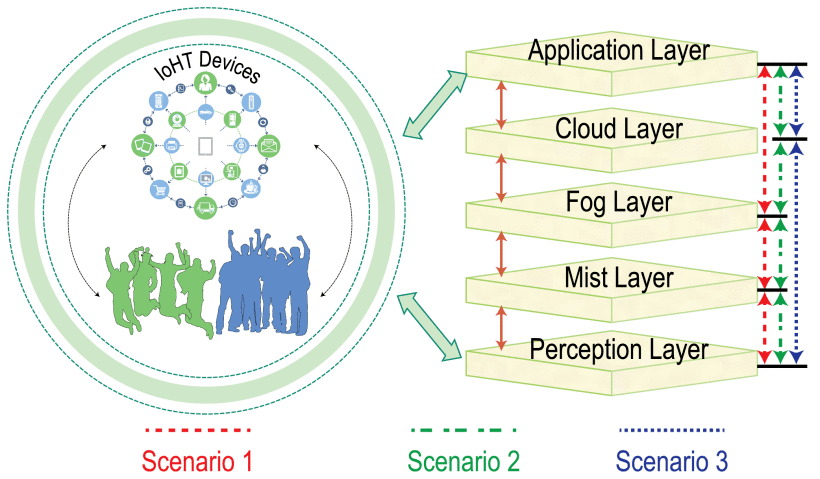
\includegraphics[width=\linewidth]{image/framework.png}
	\caption{IoHT Framework}
	\caption*{src:ASIF-UR-RAHMAN et al:\cite{3}}
\end{figure}

\subsection{The Components of 5-Layered Architecture}

\graphicspath{{C:/Users/LIKITHA/semitex/chapters}}
\begin{figure}[H]
	\centering
	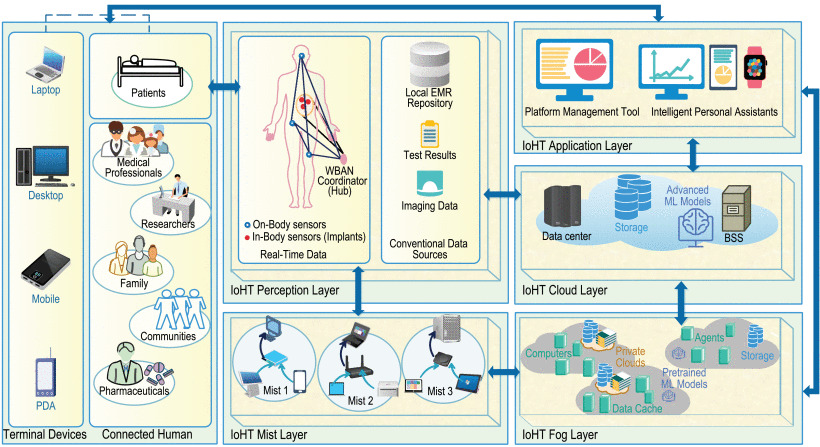
\includegraphics[width=\linewidth]{image/architecture.jpg}
	\caption{IoHT Framework Architecture}
		\caption*{src:ASIF-UR-RAHMAN et al:\cite{3}}
\end{figure}

Five Components of the framework are,\\
\begin{enumerate}
	\item Perception Layer
	\item Mist Layer
	\item Fog Layer
	\item Cloud Layer
	\item Application Layer\cite{3} 
\end{enumerate}


\subsection{Layers and their Goals}
\begin{figure}[H]
	\centering
	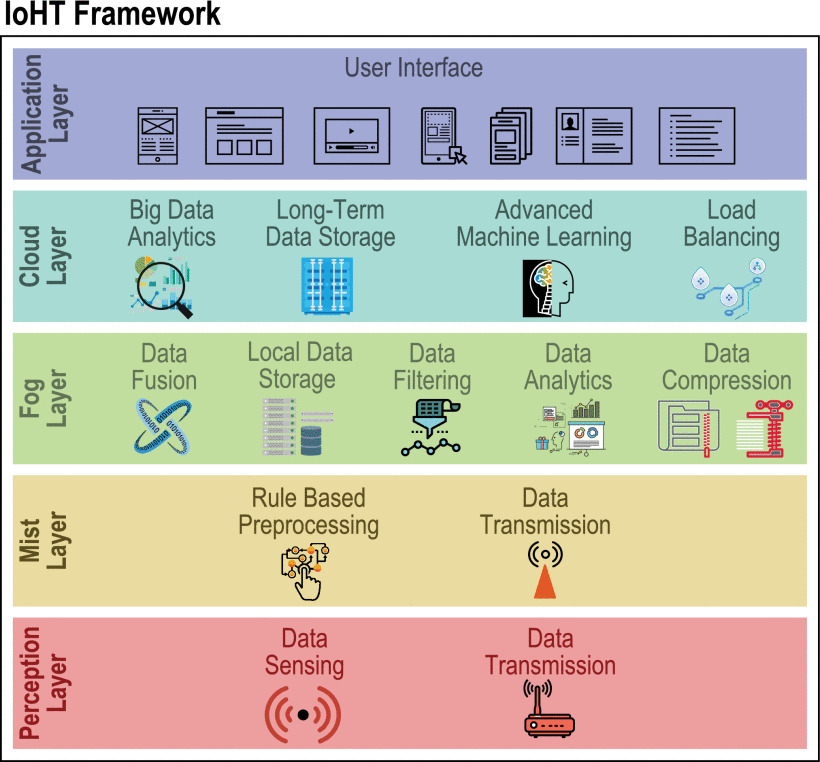
\includegraphics[width=\linewidth]{image/layered.jpg}
	\caption{Functionaities of 5-Layered IoHT Framework}
	\caption*{src:ASIF-UR-RAHMAN et al:\cite{3}}
\end{figure}

\begin{enumerate}
	\item Perception Layer:\\
	It is the lowest layer in IoHT Framework which identifies the devices that is connected to transmission and data gathering devices such as sensors,RFID tags,readers,medical imaging devices,etc which is inturn connected to the network and collects the data which is real-time as well as non-real time data.Otherthan realtime data there exists healthcare Big data such as (non)medical imaging data,electronic medical record(eMR),unstructured clinical notes etc which requires special handling because of their requirement of advanced data analytics.Based on the data type and processing requirements ,both kinds of healthcare data is transmitted to the next layer either to the Mist or Fog or Cloud\cite{3}.\\
	\item Mist Layer:\\
	In order to deal with critical time data processing,Mist was introduced in the model which stays inside the network fabric and operates at the edge of the network using sensors and actuator controllers and performs prepocessing based on rule based sensor data\cite{3}.Mist is responsible for optiml resource utilization of Things that have limited power,memory and communication bandwidth at the edge of IoT network.\\
	\item Fog Layer:\\
	In order to detect the anomalies(irregularities) and take immediate necessary actions by providing quick alarms at real time,Fog Layer was introduced.The fog layer is a decentralized architecture which ensures minimal latency and high responsiveness by bringing computing resources and application servers close together to the edge\cite{3}.This reduces latency and load on the cloud by local data storage,data compression,data filtering and intermediate data analytics that will improve QoS,System performance and save bandwidth.\\
	\item Cloud Layer:\\
	All healthcare data from fog layer and nonsensor sources such as eMR,eHR etc gets combined at Cloud layer for long-term storage, and big data and advanced analytics.The Cloud Layer is capable of connecting to Fog layer,Application layer and perception layer\cite{3}.It performs data analytics including machine learning,rule based processing,data mining and reasoning based algorithm to abstract meaningful data from healthcare data.\\
	\item Application Layer:\\
	It is the top most layer in IoHT framework that provides user interface between different stake holders and frameworks delivering many healthcare applications to the stakeholders and application developers by providing accesss according to the right and privilege from the cloud or fog layer directly\cite{3}.
\end{enumerate}

\subsection{Data processing \& Storage}
\subsubsection{Data-centric perspective}\\
\hfill\\ \\
In order to ensure smooth connectivity of heterogeneous data,a data centric transmission scheme has been made use of in the five-layered architecture.\\ \\
Depending on the availability of resource and data traffic,the processing load is assigned to either Mist or Fog or Cloud based on rule based Preprocessing, big data analytics,machine learning and etc in the 5-layered architecture.\\

The Below Flowchart describes the data transmission and processing that takes place at different layers of the IoHT Framework\cite{3}.\\

\begin{figure}[H]
	\centering
	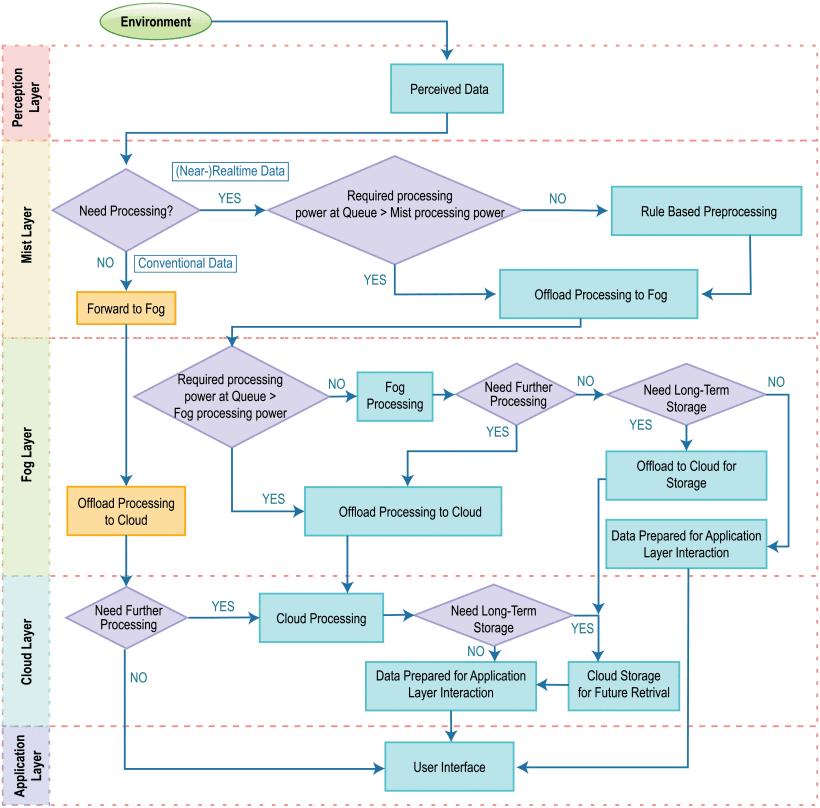
\includegraphics[width=\linewidth]{image/Datatransmission.png}
	\caption{Flowchart of data transmission and processing}
	\caption*{src:ASIF-UR-RAHMAN et al:\cite{3}}
\end{figure}

In order to achieve consistent communication among the heterogeneous data that is generated from perception layer in the proposed IoHT Framework,a data centric transmission scheme was maintained in order to deal with different types of data that was generated such as real time,near real time and offline mode(batch mode/Big data).To processing this data,it takes place in two different paths based on the traffic of data and availability of resource to attain better QoS,reduced latency and optimized power consumption\cite{3}.\\ \\

In case of real-time data,the data that is generated from the sensors that are located in the closest region and is first sent to Mist layer for processing and then forwarded to the next layer Fog which can deal with intermediate analytics and then the results are sent to application layer.

When the intermediate results sent by Fog layer is not sufficient,data is offloaded to the cloud layer which is capable of handling big data analytics,advanced machine learning,massive data generated by advanced medical instruments and etc and the data get stored in cloud for long term data storage that can be used further for reference.\\


\subsubsection{Networking}
The heterogeneous data generated from perception layer that can be real-time and non real time is sent to the nearest IoT hubs for processing.According to the processing rules and data traffic,it is then forwarded to either Mist or Fog or Cloud for preprocessing.In this process,the most critical aspect is to maintain QoS and that is achieved by deploying SDN(Software Defined Network)a programmable network structure that works on IoHT framework as centralized or decentralized for resource allocation,scheduling,routing and flow control through SDNC that uses network virtualization by decoupling control plane from data plane\cite{3}.\\

To attain better QoS,the network traffic is prioritized based on the transmission rate and delay and is classified as Delay-sensitive(DS),loss-sensitive(LS) and both delay as mixed(M)\cite{3}.\\

A sample data of IoHT healthcare traffic classification is as shown below.\\

\begin{figure}[H]
	\centering
	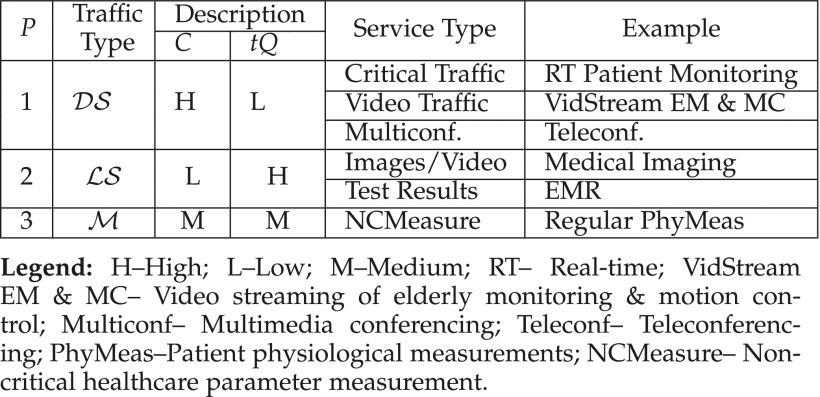
\includegraphics[width=\linewidth]{image/Table.png}
	\caption{Flowchart of data transmission and processing}
	\caption*{src:ASIF-UR-RAHMAN et al:\cite{3}}
\end{figure}
\newpage
\subsection{Data Analytics \& Machine Learning}
With the evolution of IoHT in recent years,traditional databases cannot handle the huge data and there is a huge hype for Machine Learning methodologies and Data Analytics to be used to deal with the voluminous data generated by the sensors and IoHT devices in order to provide useful and innovative process to the industries for cost cutting and improved approaches helping their business models achieve a better experience by enabling a parallel execution and distribution of data on multiple servers.\\ \\
The voluminous data generated by the IoHT devices require special methods and approach for handling and processing the structured and unstructured data.Machine learning plays an important role in IoHT Framework which is capable of handling the decisions based on certain Machine learning alogorithms where it can provide services with faster analysis and expert intervention for better treatment recommendations for the monitor of diseased person.By using machine learning methods in devices,it firstly works towards the goal irresppective of the factors that can impede and later decides the important input variables required to achieve the goal and predict the future events ensuring prevention before hand.\cite{syed2019data}\\ \\
Although data analytics could be made use of for measuring success overtime by providing smarter decision and generates report based on the data that was collected,it is not appropriate for IoT as data analytics is often static having limited-use in addressing fast-changing and unstructured data.\cite{calum}But Machine learning addresses the fast changing and unstructured data by focusing on the outcome fisrt and later decides automatically which variables is required and their interactions accordingly based on certain algorithm implementation.\\ \\
Machine Learning is not just used for machines and devices where maintainence is automated but humans too,for calling an emergency support automatically when in need.\\ \\

Example :\\ Diastolic/sistolic pressure alert event\\
High Blood pressure is one of the crucial factors that leads to stroke.Hence continous monitoring of blood pressure anytime anywhere is very essential in order to prevent and predict stroke before hand.\cite{ma2014blood} According to one of the research,a calibration method using machine learning algorithms was made use of in order to detect the variation of pulse transit time by detecting automatically the compensatory movements based on sensors and camera based devices around the patient.By continuously monitoring the patient,with an average of 0.5$\pm$3.9mmHg for systolic and diastolic blood pressure\cite{ma2014blood},an aleart event will be sent when it reaches the above average blood pressure to the caretaker through the monitoring tool that can ensure high prevention and help well in hand.
